\blackslidetext{
  \centering\Large\bf Computational PPI Prediction 
}

\begin{frame}[fragile]
  \frametitle{Computational PPI Prediction}
  \framesubtitle{Datasets}

  \begin{columns}
    \begin{column}{\textwidth}
      \vspace{-2em}

      \begin{itemize}
        \item<1-> We need information about the proteins we are working with:
              \begin{itemize}
                \item sequence (FASTA),
                \item structure (PDB, mmCIF),
                
              \end{itemize}
        \item<2-> We also need labeled PPI data:
              \begin{itemize}
                \item labeled pairs of proteins,
                \item interaction netowork/graph (adjacency matrix).
              \end{itemize}
      \end{itemize}
    \end{column}
  \end{columns}

\end{frame}


\begin{frame}[fragile]
  \frametitle{Computational PPI Prediction}
  \framesubtitle{Datasets}

  \begin{columns}
    \begin{column}{0.5\textwidth}
      \centering
      \resizebox{\textwidth}{!}{
\begin{tabular}{l r r}
    \toprule
    \textbf{Database} & \textbf{Interactions} & \textbf{Sequences}\\
    \midrule
    BioGRID  & 2,911,104 & 91,289 \\
    IntAct & 1,726,205 & 145,895 \\
    STRING & 27,541,372,832 & 59,309,604 \\
    MINT &  137,544 & 27,555 \\
    Mentha & 741,337 & 90,905\\
    Negatome Database 2.0 & 6,532 & \(\approx\) 1,900\\
    Bernett Gold Standard & 274,500 & \(\approx\) 14,077 \\
    \bottomrule
  \end{tabular}
}
    \end{column}

    \begin{column}{0.5\textwidth}
      \centering
      \resizebox{\textwidth}{!}{
      \begin{tabular}{l r r}
    \toprule
    \textbf{Database} & \textbf{Proteins} & \textbf{Most represented}\\
    \midrule
    UniProt & 199,579,900 & Homo sapiens \\ 
    PDB (Experimental) &  246,045 & Homo sapiens \\ 
    AlphaFold DB &  241,070,489 & Glycine max \\ 
    RefSeq & 427,129,536 & Bacteria \\ 
    \bottomrule
  \end{tabular}
}
    \end{column}
  \end{columns}

\end{frame}

\begin{frame}[fragile]
  \frametitle{Computational PPI Prediction}
  \framesubtitle{Protein Encoding}

  \begin{columns}
    \begin{column}{0.618\textwidth}
      \vspace{-2em}

      \begin{itemize}
        \item<1-> Computers don't speak ``protein''. 
              \begin{itemize}
                \item Sequences (or structure) need to be translated to numerical values before being processed.
              \end{itemize}
        \item<2-> Some common encoding methods include:
              \begin{itemize}
                \item one-hot encoding,
                \item conjoint triad (CT),
                \item autocovariance (AC).
              \end{itemize}
      \end{itemize}
    \end{column}

    \begin{column}{0.382\textwidth}
      \flushright
      \centering
      \vfill
      \vbox to 0.35\textheight{ 
        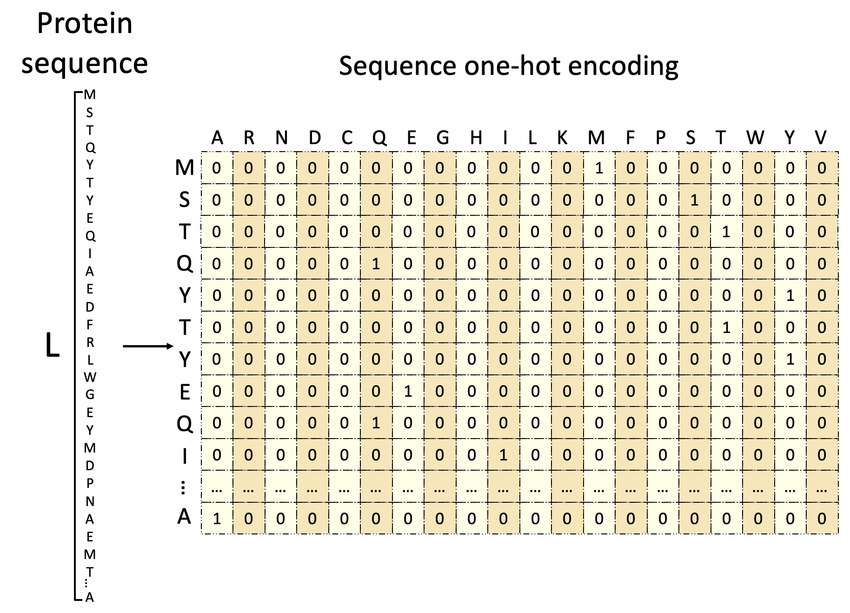
\includegraphics[width=\textwidth]{figs/pencoding.png}
      }

      {
        \vspace{2.5em}
        {\footnotesize One-hot encoding of a protein sequence\footnotemark}
        \par
      }
    \end{column}
  \end{columns}
\footnotetext{Source: https://www.researchgate.net/figure/Protein-sequence-one-hot-matrix\_fig4\_359701535}
\end{frame}

\begin{frame}[fragile]
  \frametitle{Computational PPI Prediction}
  \framesubtitle{Protein Encoding}

  \begin{columns}
    \begin{column}{\textwidth}
      \vspace{-2em}

      \begin{itemize}
        \item<1-> We need information about the proteins we are working with:
              \begin{itemize}
                \item sequence (FASTA),
                \item structure (PDB, mmCIF),
                
              \end{itemize}
        \item<2-> We also need labeled PPI data:
              \begin{itemize}
                \item labeled pairs of proteins,
                \item interaction netowork/graph (adjacency matrix).
              \end{itemize}
      \end{itemize}
    \end{column}
  \end{columns}

\end{frame}
